\documentclass[10pt]{article}
\usepackage{icmlko}

\icmlmeta{IP 파운데이션 월드모델}{220}{천장이 낮은 것과 값이 없는 것은 다르다}{노트 218이 요구한 천장 표를 만들었다. 그 표로 남은 갈래를 심사하려다, 표가 혼자서는 잘못 심사한다는 것을 알았다}

\begin{document}

\twocolumn[
\icmlheader

\begin{abstract}
노트 218이 ``무리를 손보기 전에 그 무리의 천장을 먼저 계산하라''를 남겼고
노트 219가 그것으로 남은 갈래를 심사하겠다고 적었다. 만들었다. 무리 다섯을
각각 빼서 잰 천장은 \textbf{공유 $+$0.1210 · 검색 $+$0.0365 · 위키
$+$0.0127 · 달력 $+$0.0040 · 기타 $+$0.0000} 이다. \textbf{달력이
$+$0.0040 이다} --- 노트 218이 결손을 통째로 메우고 실측한 $+$0.0001 과
맞고, \textbf{여덟 노트를 쓴 무리의 천장이 그것이었다.} 첫 수치는
아티팩트였다 --- ``단독'' 열에서 기타가 $+$0.5037 로 판 전체($+$0.4396)를
넘었는데, \textbf{기타는 게임에만 있는 축 넷이라 그 수는 게임 혼자
값}(유보 180 건)이고 분모가 다르다. 증분 열은 같은 분모라 유효하다.
그다음이 이 노트의 본론이다. 검색 천장 $+$0.0365 를 도메인별로 쪼개
갈래(``모바일 · 게임 검색 덮음 30$\sim$41\%'')를 심사했더니
\textbf{덮음과 천장이 아무 관계가 없다} --- 모바일은 덮음 54.2\% 에 천장
$+$0.0669 인데 \textbf{게임은 덮음 36.7\% 에 천장 $-$0.0014} 다. 그대로
읽으면 ``게임은 채워도 소용없다''가 된다. \textbf{틀렸다.} 덮인 66 건에서만
축과 라벨의 상관을 재니 게임이 \textbf{$+$0.508}(모멘텀) · $+$0.418(수준)
으로 \textbf{전 도메인 최고}다 --- 모바일 $+$0.332 · 웹툰 $+$0.220 · 애니
$+$0.194 보다 높다. \textbf{게임에서 검색은 정보가 없는 것이 아니라 셋에
하나만 있어서 순위를 못 바꾼다.} 중복도 아니다 --- 게임 전용 축 넷을 빼도
천장이 $-$0.0014 그대로다. 반대쪽도 갈랐다: 아이돌 천장 $+$0.0881 은
\textbf{유보 25 건짜리 잡음}이고(덮인 유보가 \emph{한 건}이다), 모바일
$+$0.0669 와 도서 $+$0.1153 은 값에서 나오며 지표는 오히려 해롭다
(지표를 끄면 각각 $+$0.0024 · $+$0.0111 오른다). \textbf{규약을 고친다} ---
천장 하나로 심사하면 안 되고 \textbf{천장 · 덮음 · 덮인 곳 상관} 세 수를
같이 봐야 한다. 천장은 ``지금 이 덮음에서 얼마''지 ``채우면 얼마''가 아니다.
\end{abstract}
]

\begin{figure*}[t]
\centering
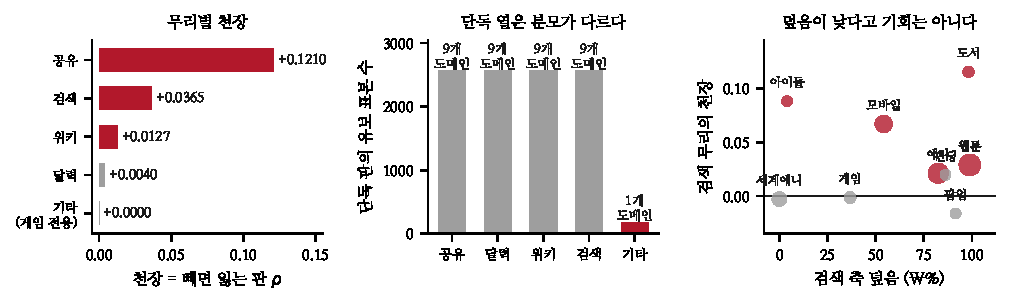
\includegraphics[width=\textwidth]{figs/ceiling.pdf}
\caption{왼쪽 --- 무리별 천장. 가운데 --- 단독 열은 분모가 다르다.
오른쪽 --- 덮음이 낮다고 기회는 아니다.}
\end{figure*}

\section{천장 표}

\begin{table}[t]
\centering\tsize
\caption{무리를 빼면 잃는 판 $\rho$(능형·트리 중 나은 쪽). 판 $+$0.4396.}
\begin{tabular}{lrrr}
\toprule
& 단독 & 뺐을 때 & \textbf{천장} \\
\midrule
\textbf{공유} & .3723 & .3186 & \textbf{$+$.1210} \\
\textbf{검색} & .2494 & .4031 & \textbf{$+$.0365} \\
위키 & .1558 & .4269 & $+$.0127 \\
\textbf{달력} & .1036 & .4356 & \textbf{$+$.0040} \\
기타(게임 전용) & \emph{.5037} & .4396 & $+$.0000 \\
\bottomrule
\end{tabular}
\end{table}

\claimx{\textbf{달력의 천장이 $+$0.0040 이다.} 노트 218이 능형의 결손을
통째로 메우고 실측한 판 변화가 $+$0.0001 이었다 --- \textbf{맞는다.}}
{\textbf{그 무리에 노트를 여덟 개 썼다}(186 · 190 · 207 · 213 · 214 ·
215 · 217 · 218). 이 표가 한 시간이면 나오는데 그것을 먼저 안 쟀다.}

\claimx{\textbf{``단독'' 열의 기타 $+$0.5037 은 아티팩트다} --- 기타는
게임에만 있는 축 넷이라 그 수는 게임 혼자 값(유보 180 건)이고 판
전체(2,565 건)와 분모가 다르다.}{\textbf{증분 열은 같은 분모라 유효하다.}
분모 가드가 잡는 모양인데 표를 만들 때는 안 붙였다 --- \textbf{표에도
가드가 필요하다.}}

\section{덮음과 천장은 관계가 없다}

\begin{table}[t]
\centering\tsize
\caption{검색 무리를 도메인별로.}
\begin{tabular}{lrrrr}
\toprule
& 유보 & 덮음 & 천장 & 덮인 곳 $|r|$ \\
\midrule
\textbf{도서} & 163 & 98.2\% & \textbf{$+$.1153} & $+$.311 \\
\textbf{모바일} & 441 & 54.2\% & \textbf{$+$.0669} & $+$.332 \\
\emph{아이돌} & \emph{25} & 4.0\% & \emph{$+$.0881} & --- \\
웹툰 & 711 & 98.9\% & $+$.0289 & $+$.220 \\
애니 & 606 & 82.5\% & $+$.0211 & $+$.194 \\
펀딩 & 80 & 86.2\% & $+$.0197 & $+$.093 \\
\textbf{게임} & 180 & 36.7\% & \textbf{$-$.0014} & \textbf{$+$.508} \\
팝업 & 59 & 91.5\% & $-$.0162 & $+$.176 \\
세계애니 & 300 & 0.0\% & $-$.0028 & --- \\
\bottomrule
\end{tabular}
\end{table}

\claimx{\textbf{게임은 덮음 36.7\% 에 천장 $-$0.0014 인데, 덮인 66 건에서
상관이 전 도메인 최고다}($+$0.508 모멘텀 · $+$0.418 수준). 모바일 $+$0.332
· 웹툰 $+$0.220 · 애니 $+$0.194 보다 높다.}{\textbf{정보가 없는 것이
아니라 셋에 하나만 있어서 순위를 못 바꾼다.} 천장만 보고 ``게임은 채워도
소용없다''로 읽으면 정확히 반대로 심사한다.}

\claimx{\textbf{중복도 아니다} --- 게임 전용 축 넷(가격 · 연령등급 등)을
빼도 검색 천장이 $-$0.0014 그대로다.}{첫 설명은 ``게임에는 자기 축이 있어
검색이 잉여''였는데 \textbf{그것이 아니다}(노트 133 --- 첫 설명을 그대로
안 쓴다).}

\begin{table}[t]
\centering\tsize
\caption{검색이 덮인 행에서만 재면 --- ``채웠을 때''의 대리.}
\begin{tabular}{lrrrr}
\toprule
& 있을 때 & 뺐을 때 & 천장 & n \\
\midrule
\textbf{게임} & .6649 & .6240 & \textbf{$+$.0409} & 66 \\
\textbf{모바일} & .5117 & .4159 & \textbf{$+$.0957} & 239 \\
\bottomrule
\end{tabular}
\end{table}

\claimx{\textbf{덮인 행에서만 재면 게임의 천장이 $-$0.0014 에서
$+$0.0409 가 된다.} 모바일도 $+$0.0669 에서 $+$0.0957 로 오른다.}
{\textbf{덮음이 문제고 정보가 아니라는 직접 증거다.} 이 수가 ``채우면
얼마''의 대리이고, 천장 표가 혼자서는 못 주는 수다.}

\section{반대쪽도 갈랐다}

\begin{table}[t]
\centering\tsize
\caption{지표인가 값인가(검색 지표를 상수로 묶으면).}
\begin{tabular}{lrrr}
\toprule
& 그대로 & 지표 끔 & 검색 뺌 \\
\midrule
\emph{아이돌} & .2301 & .2105 & .1420 \\
모바일 & .5570 & \textbf{.5594} & .4901 \\
도서 & .3125 & \textbf{.3236} & .1972 \\
\bottomrule
\end{tabular}
\end{table}

\claimx{\textbf{아이돌 $+$0.0881 은 잡음이다} --- 유보 25 건이고 그중 검색이
덮인 것이 \emph{한 건}이다. $n{=}25$ 에서 스피어만의 SE 가 $\approx$0.20
이라 $+$0.088 은 안쪽이다.}{\textbf{천장 표에 표본 수를 같이 안 적으면
이런 줄을 기회로 읽는다.} 노트 183의 그늘 가드가 도메인별 하락을 보는데,
\emph{상승}도 작은 도메인에서는 똑같이 못 믿는다.}

\claimx{\textbf{모바일과 도서는 값에서 나온다} --- 지표를 끄면 오히려
$+$0.0024 · $+$0.0111 오른다.}{\textbf{한철 가드가 잡는 모양의 반대다} ---
여기서는 지표가 해롭기만 하다. 값이 실린 무리에서는 결측 무늬가 잡음이다.}

\section{규약을 고친다}

\claimx{\textbf{천장 하나로 심사하면 안 된다.} 천장은 ``지금 이 덮음에서
얼마''지 ``채우면 얼마''가 아니다 --- 덮음이 낮은 무리에서 천장은 기회를
\emph{감춘다.}}{\textbf{세 수를 같이 본다: 천장 · 덮음 · 덮인 곳 상관.}
그리고 표본 수. 넷이 다 있어야 ``채울 값이 있나''를 판단할 수 있다.}

\begin{table}[t]
\centering\tsize
\caption{갈래 심사 결과.}
\begin{tabular}{lll}
\toprule
& 판단 & 까닭 \\
\midrule
\textbf{게임 검색} & \textbf{채운다} & 덮인 곳 $+$.508 · 덮음 37\% \\
\textbf{모바일 검색} & \textbf{채운다} & 천장 $+$.067 · 덮음 54\% \\
세계애니 검색 & 못 잰다 & 덮음 0\% \\
아이돌 검색 & 보류 & 유보 25 건 \\
달력 & 닫는다 & 천장 $+$.0040 \\
\bottomrule
\end{tabular}
\end{table}

\begin{table}[t]
\centering\tsize
\caption{남은 것.}
\begin{tabular}{ll}
\toprule
\textbf{게임 제목} & 영문 제목으로 다시 긁으면 덮음이 오르나 \\
\textbf{모바일 제목} & 같은 물음 --- 54\% $\to$ 얼마까지 \\
표 가드 & 분모 · 표본 수를 표에 자동으로 붙일 것 \\
\bottomrule
\end{tabular}
\end{table}

첫 줄이 이 사이클이 가리키는 다음 수집이다. \textbf{게임 검색 덮음이
36.7\% 인 까닭은 네이버 데이터랩이 한글 질의만 받는데 스팀 게임 제목이
영문이기 때문이다}(노트 149의 언어 한계). \textbf{덮인 행에서만 잰 천장이 $+$0.0409 이므로
나머지 셋 중 둘을 채우면 게임 도메인에서 검색이 처음으로 순위를 바꾼다.} 게임은 유보 180 건으로 판의 7\% 이고, 모바일(441 건 ·
17\%)까지 합치면 검색 천장 $+$0.0365 의 상당 부분이 아직 안 쓰인 채로
있다. \textbf{이번에는 천장을 먼저 쟀으므로 그 수집이 값이 있다는 것을
쓰기 전에 안다.}

\end{document}
